\chapter{Simulation Algorithms}
\label{chapter:simulation}
In this chapter, we will give some simulations in  Matlab\textsuperscript{\textregistered} environment: Inhomogeneous Poisson Process, Intensity-based Hawkes Process, Cluster-based Hawkes Process.
\section{Simulation of Inhomogeneous Poisson Process}
The Inhomogeneous Poisson Process is given in Algorithm \ref{algorithm:poison} that is performed Matlab\textsuperscript{\textregistered} environment.
\lstinputlisting{InhomogeneousPoissonProcess.m}
\begin{example}
	\label{example:inhomogeneouspoi}
 Simulating an inhomogeneous Poisson process with intensity function $\lambda(t)=2+\sin(t)$, bounded value $M=4$ and $T=4\pi$.
\end{example}
%To simulate in the \autoref{example:inhomogeneouspoi}, we will call function as follows:
%\lstinputlisting{main_InhomogeneousPoissonProcess.m}
\begin{figure}[H]
	\centering
	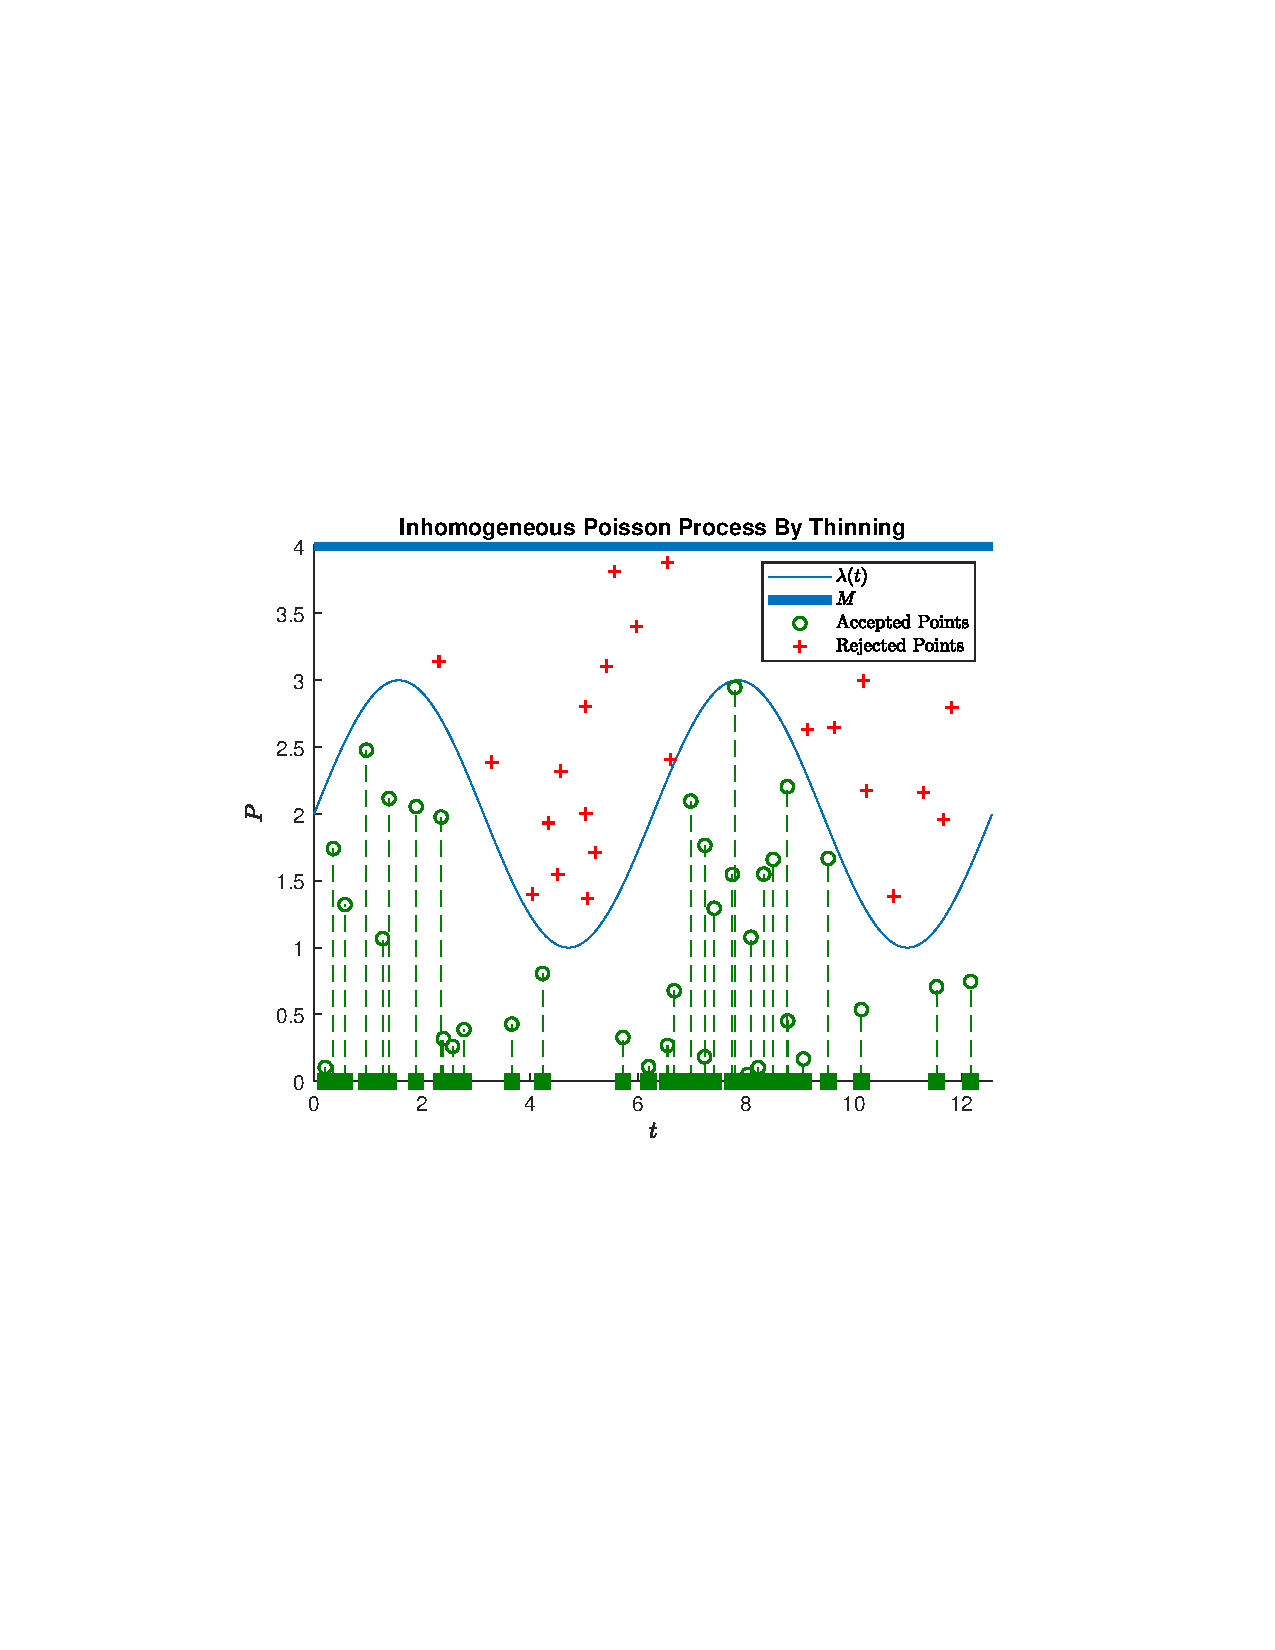
\includegraphics[trim={5cm 9cm 3.5cm 9cm},height=4.5in,width=6.5in]{inhomopoisson.pdf}
	\caption[The inhomogeneous Poisson process.]{The inhomogeneous Poisson process.}
	\label{figure:inhomopoisson}
\end{figure}
Figure \ref{figure:inhomopoisson} illustrates the result of inhomogeneous Poisson process. Each $(t,P)$ point describes a proposed arrival at time $t$ whose $P$ value. The circles are the accepted points, the plus signs are the rejected points and the squares are the point processes.
\section{Simulation of Intensity-based Hawkes Process}
The Intensity-based Hawkes Process is given in Algorithm \ref{algorithm:hawkesthinning} that is performed Matlab\textsuperscript{\textregistered} environment.
\lstinputlisting{HawkesProcessByThinning.m}
\lstinputlisting{cif.m}
\begin{example}
	\label{example:hawkesthinning}
	Simulating a intensity-based Hawkes Process with condition intensity function $(\lambda,\alpha,\beta)=(1,1,1.2)$ and $T=4$.
\end{example}
Figure \ref{figure:hawkesthinning} illustrates the result of the Intensity-based Hawkes Process in the \autoref{example:hawkesthinning}. Each $(t,P)$ point describes a proposed arrival at time $t$ whose $P$ value. The circles are the accepted points, the plus signs are the rejected points and the squares are the point processes.
%\textbf{Solution}
%To simulate in the \autoref{example:hawkesthinning}, we will call function as follows:
%\lstinputlisting{main_HawkesProcessByThinning.m}
\begin{figure}[H]
	\centering
	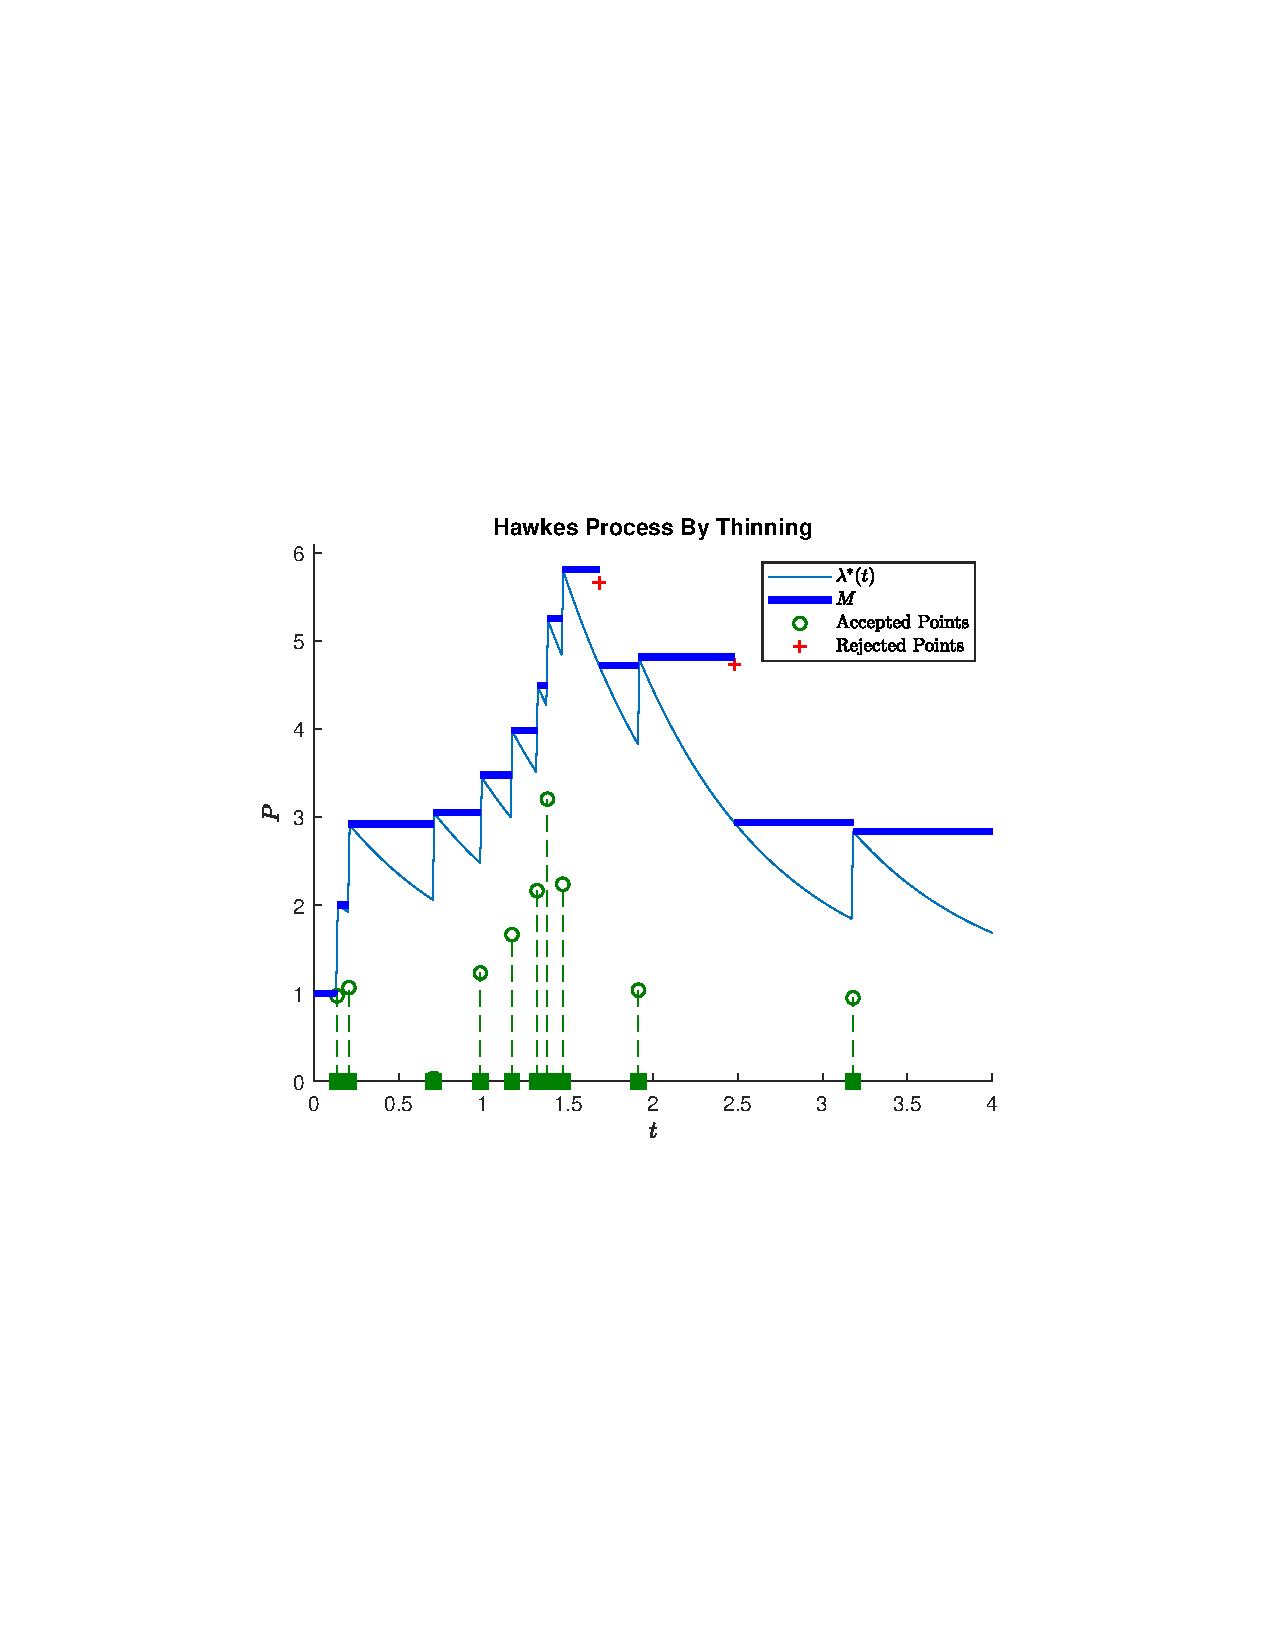
\includegraphics[trim={5cm 9cm 3.5cm 9cm},height=4.5in,width=6.5in]{hawkesbythinning.pdf}
	\caption[The Intensity-based Hawkes Process.]{The Intensity-based Hawkes Process.}
	\label{figure:hawkesthinning}
\end{figure}
\section{Simulation of Cluster-based Hawkes Process}
The Cluster-based Hawkes Process is given in Algorithm \ref{algorithm:hawkescluser} that is performed Matlab\textsuperscript{\textregistered} environment.
\lstinputlisting{HawkesProcessByClustering.m}
\begin{example}
	\label{example:hawkescluster}
	Simulating a cluster-based Hawkes Process with condition intensity function $(\lambda,\alpha,\beta)=(1,2,1.2)$ and $T=10$.
\end{example}
%\textbf{Solution}
%To simulate in the \autoref{example:hawkescluster}, we will call function as follows:
%\lstinputlisting{main_HawkesProcessByClustering.m}
\begin{figure}[H]
	\centering
	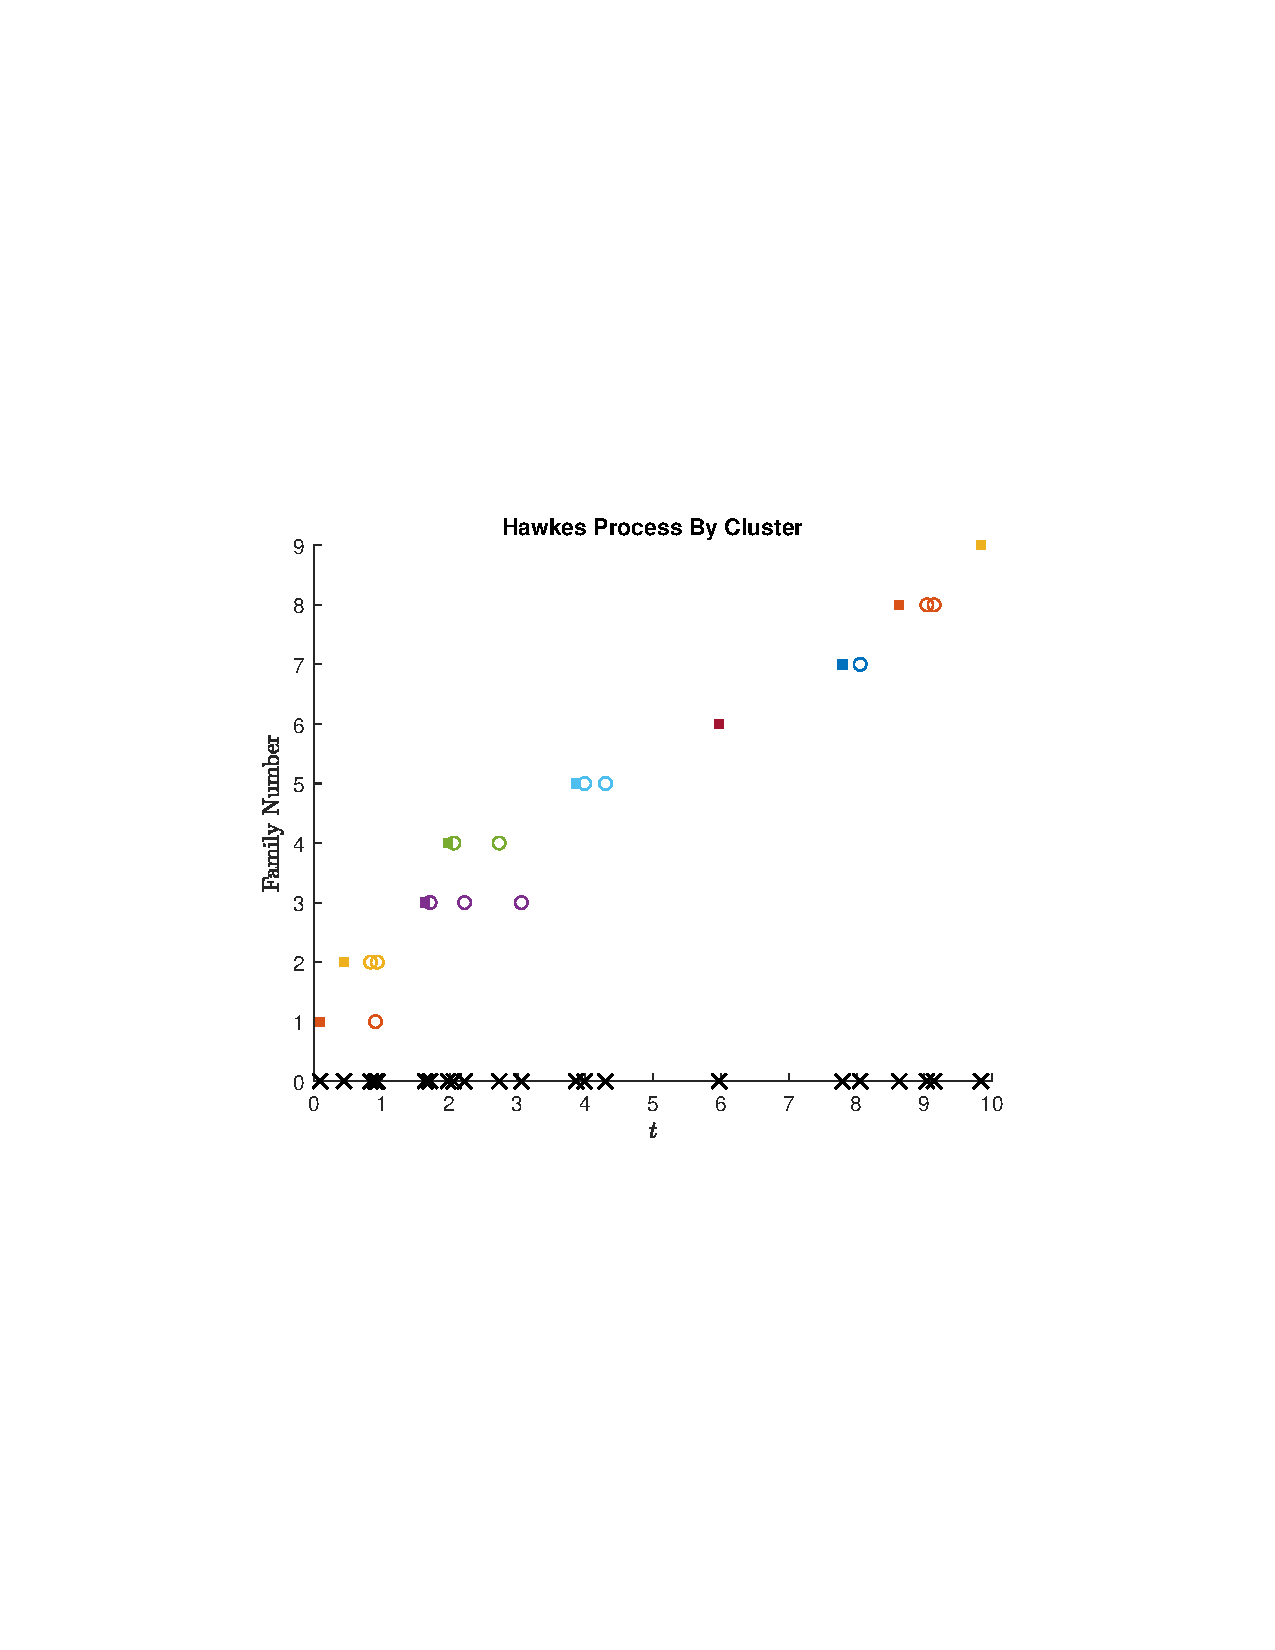
\includegraphics[trim={5cm 8.8cm 3.5cm 9cm},height=4.5in,width=6.5in]{hawkesbycluster.pdf}
	\caption[The Cluster-based Hawkes Process.]{The Cluster-based Hawkes Process.}
	\label{figure:hawkescluster}
\end{figure}
Figure \ref{figure:hawkescluster} illustrates the result of the Cluster-based Hawkes Process. The squares are the immigrant points, the circles of the same height and color are descendant of immigrant points and the crosses are the point processes.